\section{二阶线性常微分方程找特解}
\textit{Now, we want to find a special solution for following ordinary differential equation} :

\[\frac{\mathrm{d}^2 y}{\mathrm{d} x^2} + p(x) \frac{\mathrm{d} y}{\mathrm{d} x}+q(x)y=f(x) \tag{a} \]

\textit{Assume the general solution of this ordinary differential equation is} y(x)= $c_1$ $y_1$(x)+$c_2$ $y_2$(x).

\textit{Then we assume the special solution of this ordinary differential equation is} $y^*$(x)= $c_1$(x) $y_1$(x)+$c_2$(x) $y_2$(x).

\textit{Bringing this special solution} $y^*$(x) \textit{into the equation} (a) \textit{, we can get} :

\[\sum_{1}^{2} \left (\frac{\mathrm{d}^2 c_i}{\mathrm{d} x^2} y_i +2\frac{\mathrm{d} c_i}{\mathrm{d} x} \frac{\mathrm{d} y_i}{\mathrm{d} x}+ c_i \frac{\mathrm{d}^2 y_i}{\mathrm{d} x^2} + p( \frac{\mathrm{d} c_i}{\mathrm{d} x} y_i + c_i \frac{\mathrm{d} y_i}{\mathrm{d} x})+qc_iy_i \right)=f(x)\]

\[\sum_{1}^{2} \left ( (\frac{\mathrm{d}^2 c_i}{\mathrm{d} x^2} y_i +2\frac{\mathrm{d} c_i}{\mathrm{d} x} \frac{\mathrm{d} y_i}{\mathrm{d} x}+p \frac{\mathrm{d} c_i}{\mathrm{d} x} y_i + (c_i \frac{\mathrm{d}^2 y_i}{\mathrm{d} x^2}+pc_i \frac{\mathrm{d} y_i}{\mathrm{d} x}+qc_iy_i) \right)=f(x) \quad (b) \]

\textit{Since the solutions of this ordinary differential equation satisfy following equation} :

\[\sum_{1}^{2} \left ( \frac{\mathrm{d}^2 y_i}{\mathrm{d} x^2} + p(x) \frac{\mathrm{d} y_i}{\mathrm{d} x}+q(x)y_i \right ) =f(x) \tag{c}\]

\textit{We can simplify the equation} (b) :

\[\sum_{1}^{2} \left(\frac{\mathrm{d}^2 c_i}{\mathrm{d} x^2} y_i +2\frac{\mathrm{d} c_i}{\mathrm{d} x} \frac{\mathrm{d} y_i}{\mathrm{d} x}+p(x) \frac{\mathrm{d} c_i}{\mathrm{d} x} y_i) \right)=f(x) \tag{d} \]

\textit{It doesn't matter that we can assume} :

\[\sum_{1}^{2} \frac{\mathrm{d} c_i}{\mathrm{d} x} y_i =0 \tag{e} \]

\textit{We can also get following equation from equation} (e) :

\[\sum_{1}^{2} \left( \frac{\mathrm{d}^2 c_i}{\mathrm{d} x^2} y_i +\frac{\mathrm{d} c_i}{\mathrm{d} x} \frac{\mathrm{d} y_i}{\mathrm{d} x} \right)=0 \tag{f}\]

\textit{Bring equation} (e) \textit{and} (f) \textit{into equation} (d) \textit{,we can get} :

\[\sum_{1}^{2} \frac{\mathrm{d} c_i}{\mathrm{d} x} \frac{\mathrm{d} y_i}{\mathrm{d} x}=f(x) \tag{g}\]

\textit{Combine equation} (e) and \textit{equation} (g) \textit{,we can get} :

\[\begin{pmatrix} y_1 & y_2 \\ {y_1}' & {y_2}' \end{pmatrix} \begin{pmatrix} {c_1}' \\ {c_2}' \end{pmatrix} = \begin{pmatrix} 0 \\ f(x) \end{pmatrix} \tag{h} \]

\textit{Solve this system of equations, we can work out following two equations}:

\[ {c_1}'=\frac {\begin{pmatrix} 0 & y_2 \\ f(x) & {y_2}' \end{pmatrix}} {\begin{pmatrix} y_1 & y_2 \\ {y_1}' & {y_2}' \end{pmatrix}} =\frac {-y_2 f(x)}{y_1 {y_2}' - y_2 {y_1}'} \tag{i1} \]

\[ {c_2}'=\frac {\begin{pmatrix} y_1 & 0 \\ {y_1}' & f(x) \end{pmatrix}} {\begin{pmatrix} y_1 & y_2 \\ {y_1}' & {y_2}' \end{pmatrix}} =\frac {y_1 f(x)}{y_1 {y_2}' - y_2 {y_1}'} \tag{i2} \]

\textit{Finally,we can get the special solution of equation} (a) :

\[y^*=\int{\frac {-y_2 f(x)}{y_1 {y_2}' - y_2 {y_1}'}} y_1 + \int{\frac {y_1 f(x)}{y_1 {y_2}' - y_2 {y_1}'}} y_2 \tag{j} \]


\section{Wronskian行列式找特解}
找特解的时候我们一般采用常数变易法,我们假设我们要处理的线性非齐次常系数微分方程为
\[\sum_{i=0}^na_iy^{(i)}=f \qquad (\text{记} \ y^{(0)}=y) \tag{*}\]
我们记对应齐次方程(无简并特征根)的通解的常数易变为,其中$y_i(t)$满足齐次方程。
\[y(t)=\sum_{j=1}^nv_j(t)y_j(t) \tag{1}\]
将(1)将代入(*)式,得到
\[\sum_{i=0}^na_i\sum_{j=1}^n\left(\sum_{k=0}^iC_i^kv_j^{(k)}y_j^{(i-k)}\right)=f\]
按照$v_j^{(i)}$做整理得到
\[\sum_{j=1}^n\sum_{i=0}^nv_j^{(i)}\left(\sum_{k=i}^{n}a_{k}C_{k}^iy_j^{(k-i)}\right)=f\]
我们会发现,所以含$v_i^{(0)}$的项抵消了,因为$v_i^{(0)}$项的系数是下式
\[\sum_{j=1}^nv_j^{(0)}\left(\sum_{k=0}^{n}a_{k}y_j^{(k-i)}\right)=0\]
所以有
\[\sum_{j=1}^n\sum_{i=1}^nv_j^{(i)}\left(\sum_{k=i}^{n}a_{k}C_{k}^iy_j^{(k-i)}\right)=f\]
我们取含$v_j'$的项为$f$,其余的项为0。
\[\sum_{j=1}^nv_j'\left(\sum_{k=1}^{n}a_{k}C_{k}^1y_j^{(k-1)}\right)=f \qquad \sum_{j=1}^nv_j^{(i)}\left(\sum_{k=i}^{n}a_{k}C_{k}^iy_j^{(k-i)}\right)=0 \quad (i=2,3,\cdots,n)\]
改写方程
\[\sum_{k=1}^{n}\sum_{j=1}^nv_j'\left(a_{k}C_{k}^1y_j^{(k-1)}\right)=f\]
容易看出,上式可以进一步改写成
\[
\begin{pmatrix}
    a_{1}C_{1}^1y_1 & a_{1}C_{1}^1y_2 & \cdots & a_{1}C_{1}^1y_n \\
    a_{2}C_{2}^1y'_1 & a_{2}C_{2}^1y'_2 & \cdots & a_{2}C_{2}^1y'_n \\
    \vdots & \vdots & \ddots & \vdots \\
    a_{n}C_{n}^1y^{(n-1)}_1 & a_{n}C_{n}^1y^{(n-1)}_2 & \cdots & a_{n}C_{n}^1y^{(n-1)}_n
\end{pmatrix}    
\begin{pmatrix}
    v'_1 \\ v'_2 \\ \vdots \\ v'_n \\
\end{pmatrix}   
=
\begin{pmatrix}
    0 \\ 0 \\ \vdots \\ f \\
\end{pmatrix}     
\]
根据线性方程组的性质,我们知道,上式和下式的解相同:
\[
\begin{pmatrix}
    y_1 & y_2 & \cdots & y_n \\
    y'_1 & y'_2 & \cdots & y'_n \\
    \vdots & \vdots & \ddots & \vdots \\
    y^{(n-1)}_1 & y^{(n-1)}_2 & \cdots & y^{(n-1)}_n
\end{pmatrix}    
\begin{pmatrix}
    v'_1 \\ v'_2 \\ \vdots \\ v'_n \\
\end{pmatrix}   
=
\begin{pmatrix}
    0 \\ 0 \\ \vdots \\ f' \\
\end{pmatrix}     
\qquad \text{where} \ f'=\frac{f}{a_{n}C_{n}^1}=\frac{f}{na_{n}}
\]
为了保有方程的形式,我们可以重新将系数$na_n$并入一开始求算的通解中,即
\[y_j:=na_ny_j \qquad (j=1,2,\cdots,n)\]
则方程组可以写成
\[
\begin{pmatrix}
    y_1 & y_2 & \cdots & y_n \\
    y'_1 & y'_2 & \cdots & y'_n \\
    \vdots & \vdots & \ddots & \vdots \\
    y^{(n-1)}_1 & y^{(n-1)}_2 & \cdots & y^{(n-1)}_n
\end{pmatrix}    
\begin{pmatrix}
    v'_1 \\ v'_2 \\ \vdots \\ v'_n \\
\end{pmatrix}   
=
\begin{pmatrix}
    0 \\ 0 \\ \vdots \\ f \\
\end{pmatrix}     
\]
如果我们记
\[
\mathcal{W}(s)=
\begin{vmatrix}
    y_1(s) & y_2(s) & \cdots & y_n(s) \\
    y'_1(s) & y'_2(s) & \cdots & y'_n(s) \\
    \vdots & \vdots & \ddots & \vdots \\
    y^{(n-1)}_1(s) & y^{(n-1)}_2(s) & \cdots & y^{(n-1)}_n(s)
\end{vmatrix}  
\]
\[
\mathcal{W}_i(s)=
\begin{vmatrix}
    y_1(s) & y_2(s) & \cdots & y_{i-1}(s) & 0 & y_{i+1}(s) & \cdots & y_n(s) \\
    y'_1(s) & y'_2(s) & \cdots & y'_{i-1}(s) & 0 & y'_{i+1}(s) & \cdots & y'_n(s) \\
    \vdots & \vdots & \cdots & \vdots & \vdots & \vdots & \cdots & \vdots \\
    y^{(n-1)}_1(s) & y^{(n-1)}_2(s) & \cdots & y^{(n-1)}_{i-1}(s) & f(s) & y^{(n-1)}_{i+1}(s) & \cdots & y^{(n-1)}_n(s)
\end{vmatrix} 
\]
由$Cramer$法则可以知道
\[v_i'(s)=\frac{\mathcal{W}_i(s)}{\mathcal{W}(s)} \qquad (i=1,2,\cdots,n)\]
故
\[v_i(t)=\int v_i'(s)ds=\int \frac{\mathcal{W}_i(s)}{\mathcal{W}(s)}ds\]
我们也可以将$f(s)$提出,记
\[
\mathcal{W}_{0,i}(s):=f(s)
\begin{vmatrix}
    y_1(s) & y_2(s) & \cdots & y_{i-1}(s) & 0 & y_{i+1}(s) & \cdots & y_n(s) \\
    y'_1(s) & y'_2(s) & \cdots & y'_{i-1}(s) & 0 & y'_{i+1}(s) & \cdots & y'_n(s) \\
    \vdots & \vdots & \cdots & \vdots & \vdots & \vdots & \cdots & \vdots \\
    y^{(n-1)}_1(s) & y^{(n-1)}_2(s) & \cdots & y^{(n-1)}_{i-1}(s) & 1 & y^{(n-1)}_{i+1}(s) & \cdots & y^{(n-1)}_n(s)
\end{vmatrix} 
\]
则有
\[v_i(t)=\int v_i'(s)ds=\int \frac{f(s)\mathcal{W}_{0,i}(s)}{\mathcal{W}(s)}ds\]

\section{TST推导}\textit{Basic hypothesis:}

A. Before dividing surface, transition-state and reactant obey Maxwell Boltzmann distribution;

B. After dividing surface, the reaction between transition-state and product is irreversible reaction, and once molecules go through dividing surface we consider they must become product.

We call reactant as R and transition-state as TS.
\[-\frac{\mathrm{d} {[R]}}{\mathrm{d} t} = k_f[R]-k_b[TS] \tag{a}\]
\[-\frac{\mathrm{d} {[TS]}}{\mathrm{d} t} = k_2[TS]-k_f[R]+k_b[TS] \tag{b}\]

Because of hypothesis 1, we can get following equation:
\[k_f[R]-k_b[TS]=0 \qquad \Rightarrow \qquad [TS]=\frac{k_f}{k_b}[R]\]

And we consider probability flow as a constant, also the change on R and TS is relative tiny:
\[\frac{\mathrm{d} {[R]}}{\mathrm{d} t} = \frac{\mathrm{d} {[TS]}}{\mathrm{d} t}\]
then:
\[-\frac{\mathrm{d} {[TS]}}{\mathrm{d} t} = k_2[TS]+k_b[TS]-k_f[R]=k_2[TS]=\frac{k_fk_2}{k_b}[R]\]

\[-\frac{\mathrm{d} {[R]}}{\mathrm{d} t} = \frac{k_fk_2}{k_b}[R] :=k[R]\]

Since concentration is proportional to partition function, and adjust transition-state and reactant to the same energy zero point, we can write equation (b) as follows:
\[\frac{k_f}{k_b}= \frac{Q_{TS}}{Q_R} e^{\frac{E}{kT}} \tag{c} \]

Consider the neighbourhood of transition-state along reaction pathway, take a tiny length dl out, on \textit{dl} we think reaction rate is a constant approximatively. Then we can get:

\[\frac{1}{k_2}= \tau = \frac{dl}{v} = \frac{dl}{<v>} \tag {d} \]

Put equation (c) and equation (d) together, we get:

\[k= \frac{Q_{TS}}{Q_R} e^{\frac{E}{kT}} \frac{<v>}{dl} \tag{e} \]

Sinse we consider the neighbourhood of transition-state, we can consider the molecules are free particles, let's consider the one-dimension Maxwell Distribution of Speed:

\[<v> = \int_{0}^{\infty}\sqrt{\frac{\mu}{2 \pi kT}}ve^{ - \frac{\mu v^2}{2kT}}dv \tag{f} \]

Easily, we can finally get the expression of <v>:

\[<v>=\sqrt{\frac{2kT}{\pi \mu}} \tag{g}\]

Also, we can get the expression of $k$:

\[k= \frac{Q_{TS}}{Q_R} e^{\frac{E}{kT}} \sqrt{\frac{2kT}{\pi \mu}} \frac{1}{dl} \tag{h} \]

As we all know, partition function can be calculated by Hamiltonian:

\[Q_i = \sum_j<\psi_j|e^{\beta \hat{H_i}}|\psi_j>=Tr{(e^{\beta \hat{H_i}})} \quad (i=TS,R) \qquad \text{where} \quad \bra{\phi_i}\ket{\phi_j}=\delta_{ij} \tag{i}\]

We can separate transition-state's Hamiltonian as one along dividing surface and the other along reaction pathway, here we assume these two dimensions are independent:

\[Q_{TS} =Tr{(e^{\beta (\hat{H_{DS}}+\hat{H_{RP}})})}=Tr{(e^{\beta \hat{H_{DS}}})}Tr{(e^{\beta \hat{H_{RP}}})}=Q_{DS}Q_{RP} \tag{j}\]

Also, consider the molecules are free particle, and the reaction is irreverible, we get following in phase space:

\[Q_{RP}=\frac{1}{2}Q_{FP}=\frac{1}{h}\int_{-dl}^{0}\int_{-\infty}^{\infty}e^{\frac{p^2}{2 \mu kT}}dxdp \tag{k}\]

Then ,we get:

\[Q_{RP}=\frac{dl}{2h}\sqrt{2 \pi \mu kT} \tag{l} \]

Finally, we get the expression of $k$ as follows:

\[k=\frac{kT}{h} \frac{Q_{DS}}{Q_R} e^{\frac{E}{kT}} \tag{*} \]

By the way, the energy E here refers to the differential value between transition-state's vibrational level zero energy point and reaction's.

\section{随机游走均方末端距}
对于流体中某面元上的扩散速率,我们知道其正比于该流体的数量密度对运动位移矢量的偏导:
\[J=-D\nabla\rho \tag{a}\]

我们采用拉格朗日法研究扩散时,溶质密度随时间的变化,这里我们给出密度在拉格朗日法下的函数表示:
\[\rho=\rho(\vec{x},t)\]

在$\vec{x}$方向上我们考虑体积元$Ad\vec{x}$内的密度变化,在体积元中,我们可以得知,扩散速率场与面元的乘积未体积元中粒子数的变化量,与密度随时间的变化成正比,系数为-1:
\[\frac{\partial \rho}{\partial t}=-\lim_{\partial \vec{x} \rightarrow 0} \frac{[J(\vec{x}+\partial \vec{x})-J(\vec{x})] \cdot A}{\partial \vec{x} \cdot A} =-\nabla \cdot J \tag{b}\]

结合(a)、(b)两式,我们可以得到含时的扩散方程(time-dependent diffusion equation):
\[\frac{\partial \rho}{\partial t}=D\nabla^2\rho \tag{c}\]

这里我们认为扩散的体系是各向同性的,则扩散系数为一常数,反之则为$\vec{x}$的函数。

函数$\rho(\vec{x},t)$处理起来不便,我们可以考虑对其分量进行处理并使用傅里叶变换在其动量空间上进行处理,下列$x$与$k$表示沿着同一分量的位移与动量:

\[\rho(x,t)=\int_{-\infty}^{+\infty}\rho_k(t)e^{-ikx}dk\]

\[\frac{\partial \rho}{\partial t}=\int_{-\infty}^{+\infty}\frac{\mathrm{d} \rho_k(t)}{\mathrm dt}e^{-ikx}dk\]

\[\nabla^2\rho=\int_{-\infty}^{+\infty}\rho_k(t)\nabla^2 e^{-ikx}dk=\int_{-\infty}^{+\infty}-k^2\rho_k(t)e^{-ikx}dk\]

易得:
\[\int_{-\infty}^{+\infty}(\frac{\mathrm{d} \rho_k(t)}{\mathrm dt}+Dk^2\rho_k(t))e^{-ikx}dk=0\]

由$t$的任意性,我们可以得到:
\[\frac{\mathrm{d} \rho_k(t)}{\mathrm dt}+Dk^2\rho_k(t)=0 \tag{d}\]

解该微分方程我们得到以下结果:
\[\rho_k(t)=\rho_k(0)e^{-Dk^2t}\]

其中$\rho_k(0)$可以通过边界条件$\rho(\vec{0},0)=\delta(0)$确定:

\[\rho_k(t)=\frac{1}{2\pi}\int_{-\infty}^{+\infty}\rho(x,t)e^{ikx}dk\]

\[\rho_k(0)=\lim_{t \rightarrow 0}\rho_k(t)=\lim_{t \rightarrow 0}\frac{1}{2\pi}\int_{-\infty}^{+\infty}\rho(x,t)e^{ikx}dk\]

\[\lim_{t \rightarrow 0}\frac{1}{2\pi}\int_{-\infty}^{+\infty}\rho(x,t)e^{ikx}dk=\frac{1}{2\pi}\int_{-\infty}^{+\infty}\lim_{t \rightarrow 0}\rho(x,t)e^{ikx}dk\]

\[\frac{1}{2\pi}\int_{-\infty}^{+\infty}\lim_{t \rightarrow 0}\rho(x,t)e^{ikx}dk=\frac{1}{2\pi}\int_{-\infty}^{+\infty}\delta(0)e^{ikx}dk=\frac{1}{2\pi}e^{ik\vec{0}}=\frac{1}{2\pi}\]

\[\rho_k(t)=\frac{1}{2\pi}e^{-Dk^2t} \tag{e}\]

接下来进行傅里叶变换还原所得结果:

\[\rho(x,t)=\int_{-\infty}^{+\infty}\rho_k(t)e^{-ikx}dk=\int_{-\infty}^{+\infty}\frac{1}{2\pi}e^{-Dk^2t} e^{-ikx}dk\]

通过变形上式可变成:

\[\rho(x,t)=\int_{-\infty}^{+\infty}\frac{1}{2\pi}e^{-Dk^2t-ikx}dk=\int_{-\infty}^{+\infty}\frac{1}{2\pi}e^{-Dt(k+\frac{ix}{2Dt})^2-\frac{x^2}{4Dt}}dk\]

\[\rho(x,t)=\frac{1}{2\pi}e^{-\frac{x^2}{4Dt}}\int_{-\infty}^{+\infty}e^{-Dt(k+\frac{ix}{2Dt})^2}dk\]

\[\rho(x,t)=\frac{1}{2\pi}e^{-\frac{x^2}{4Dt}}\int_{-\infty}^{+\infty}e^{-Dtu^2}du=\sqrt{\frac{1}{4\pi Dt}}e^{-\frac{x^2}{4Dt}} \tag{f}\]

至此,我们得到了非定常扩散的数量密度分布,我们可以用其来求取期望:

\[<\vec{x}>=\left (\int_{-\infty}^{+\infty}x\rho(x,t)dx,\int_{-\infty}^{+\infty}y\rho(y,t)dy ,\int_{-\infty}^{+\infty}z\rho(z,t)dz \right )=\vec{0}\]\

由对称性:

\[<\vec{x}^2>=<x^2+y^2+z^2>=<x^2>+<y^2>+<z^2>=3<x^2>\]

因此有:

\[<\vec{x}^2>=3<x^2>=3\int_{-\infty}^{+\infty}x^2\rho(x,t)dx=3 \sqrt{\frac{1}{4\pi Dt}}\int_{-\infty}^{+\infty}x^2e^{-\frac{x^2}{4Dt}}dx\]

再令$w=\frac{x^2}{4Dt}$,则有:

\[<\vec{x}^2>=3\sqrt{\frac{1}{4\pi Dt}}\int_{0}^{+\infty}\sqrt{4Dtw}e^{-w}(4Dt)dw=\frac{12Dt}{\sqrt{\pi}}\int_{0}^{+\infty}\sqrt{w}e^{-w}dw\]

已知:

\[\int_{0}^{+\infty}\sqrt{w}e^{-w}dw=\Gamma(\frac{3}{2})=\frac{\sqrt{\pi}}{2}\]

最终我们得到:

\[<\vec{x}^2>=\frac{12Dt}{\sqrt{\pi}} \cdot \frac{\sqrt{\pi}}{2}=6Dt \tag{*}\]

\section{一阶微扰理论}
\subsection{一阶非简并定态微扰理论}
假定已经解出了无微扰时的薛定谔方程$H_0 \varPsi_n^0 =E_n^0 \varPsi_n^0$,我们将要利用该方程的解去求解受微扰影响后的新方程$H \varPsi_n =E_n \varPsi_n$的解。

将实际哈密顿量$H$写成如下形式,其中$H_0$为无微扰时的哈密顿量、$\lambda$为一可变参量(稍后我们会将其取为1)、$H^{'}$为微扰:
\[H=H_0+\lambda H^{'} \tag{a}\]

在给出参数$\lambda$后,将$\varPsi_n$与$E_n$对$\lambda$做幂级数展开:
\[\varPsi_n=\sum_{i=0}^{+\infty}\varPsi_n^i\lambda^i \qquad E_n=\sum_{i=0}^{+\infty}E_n^i\lambda^i \tag{b}\]

其中$\varPsi_n^i$、$E_n^i$为$\varPsi_n$、$E_n$的$i$阶修正,其中要求$\varPsi_n^i \ (\forall \, i,n \in \mathbb{R})$相互正交,可以从$\bra{\Psi}\ket{\Psi}=1$得到。

将(a)、(b)式带入原方程可得:
\[(H_0+\lambda H^{'})\sum_{i=0}^{+\infty}\varPsi_n^i\lambda^i=\sum_{i=0}^{+\infty}E_n^i\lambda^i\sum_{i=0}^{+\infty}\varPsi_n^i\lambda^i\]

展开可得:
\[H_0 \varPsi_n^0=E_n^0 \varPsi_n^0\]
\[(H_0 \varPsi_n^1+H^{'} \varPsi_n^0)\lambda=(E_n^0 \varPsi_n^1+E_n^1 \varPsi_n^0)\lambda\]
\[\cdot\cdot\cdot\]

可以看到0阶修正就是无微扰时的方程,将一阶修正项单独取出研究:
\[H_0 \varPsi_n^1+H^{'} \varPsi_n^0=E_n^0 \varPsi_n^1+E_n^1 \varPsi_n^0 \tag{c}\]

对上式两边都内积上$\varPsi_n^0$并化简得到:

\[E_n^1=<\varPsi_n^0|H^{'}|\varPsi_n^0>\]

这是一级近似中最基本的一个结果,实际上也是量子力学中最重要的方程之一,它说明了能量的一阶修正是微扰在非微扰态中的期望。

在找到了能量的一阶修正后,利用其可以推导出波函数的一阶修正,对方程(c)做一点变形:
\[(H_0-E_n^0) \varPsi_n^1=-(H^{'}-E_n^1) \varPsi_n^0 \tag{d}\]

上式中等号右边为已知函数,该方程是关于$\varPsi_n^1$的非齐次微分方程,由于$\varPsi^0$的完备性,可以将$\varPsi_n^1$表示成如下形式:
\[\varPsi_n^1=\sum_{m \neq n}c_m^n\varPsi_m^0 \tag{e}\]

将上式带入(d)方程得到:
\[(H_0-E_n^0) \sum_{m \neq n}c_m^n\varPsi_m^0=-(H^{'}-E_n^1) \varPsi_n^0\]

在方程两边同时内积上$\varPsi_m^0$得到:
\[\sum_{m \neq n} c_m^n<\varPsi_m^0|H_0-E_n^0|\varPsi_m^0>=-<\varPsi_m^0|H^{'}-E_n^1|\varPsi_n^0>\]

经过化简,最终得到:
\[c_m^n=\frac{<\varPsi_m^0|H^{'}|\varPsi_n^0>}{E_n^0-E_m^0}\]

带入展开式(e),得到了一阶修正的波函数表达式:
\[\varPsi_n^1=\sum_{m \neq n}\frac{<\varPsi_m^0|H^{'}|\varPsi_n^0>}{E_n^0-E_m^0}\varPsi_m^0\]

值得一提的是这里处理的都是无简并的非扰动能级,从波函数一阶修正的表达式中很明显能看出原因,我们将在下面的内容中解决它。并且从实际使用来看微扰理论在给出能量的近似时是非常精确的,但对波函数的计算却不是太理想。

\subsection{一阶k重简并定态微扰理论}
求解微扰的思路是寻找一个好的非微扰态的函数基组,然后将微扰展开为该函数基下的表象,当轨道的能级出现简并的时候上述的讨论将不适用,也即是我们找不到一个好的函数基组来表征微扰(因为此时的非微扰态波函数基组并不相互独立),接下来的内容我们将着重寻找一个好的函数基组。不妨假设找到的独立的函数基为$\varPsi^0$,他来源于几个简并的轨道,由于微扰会使得原本简并的轨道发生裂分,此时我们可以将该函数基写成如下形式:
\[\varPsi^0=\sum_{i=1}^k\beta_i\varPsi_{k_i}^0\]

记:
\[\varPsi_k^0=\left (\varPsi_{k_1}^0 , \varPsi_{k_2}^0 ,\varPsi_{k_3}^0, \cdot \cdot \cdot , \varPsi_{k_k}^0\right )^T\]

根据一阶微扰对应的原方程展开项(c),我们得到:
\[H_0 \varPsi_n^1+H^{'} \varPsi^0=E_n^0 \varPsi_n^1+E_n^1 \varPsi^0\]

对上述方程两侧同时内积上$\varPsi_{k_i}^0$,得到以下方程组:
\[\sum_{j=1}^k\beta_j<\varPsi_{k_i}^0|H^{'}|\varPsi_{k_j}^0>=\beta_i E_n^1 \qquad (i=1,2 \cdot\cdot\cdot n)\]

记$W_{ij}=<\varPsi_{k_i}^0|H^{'}|\varPsi_{k_j}^0> \quad (i,j=1,2 \cdot\cdot\cdot n)$,可以将方程组写得更紧凑一些:

\[
\begin{pmatrix}
W_{11} & W_{12} & \ldots & W_{1n}\\
W_{21} & W_{22} & \ldots & W_{2n}\\
\vdots & \vdots & \ddots & \vdots\\
W_{n1} & W_{n2} & \ldots & W_{nn}\\
\end{pmatrix}
\begin{pmatrix}
\beta_1\\
\beta_2\\
\vdots\\
\beta_n\\
\end{pmatrix}
=E_n^1
\begin{pmatrix}
\beta_1\\
\beta_2\\
\vdots\\
\beta_n\\
\end{pmatrix}
\tag{f} \]

求解方程组(f)实际上就是研究矩阵$(W_{ij})$的正交对角化,假设$(W_{ij})$正交对角化形式如下:
\[W=P^T \Lambda P\]

则$E_n^1$可表示成:
\[E_n^1=\Lambda\]

则事先假定的好的函数基$\varPsi^0$也就可以表示成:
\[\varPsi^0=P^T \varPsi^0_k\]

\subsection{一阶含时微扰理论}
当考虑一些更实际的体系如原子吸收与原子发射时,会遇到哈密顿量中的含时项不可忽略的情况,这时求解该体系就需要考虑含时的薛定谔方程。由于时间项的引入,简并态出现的可能性将大大下降,因此这里我们仅讨论无简并的一阶含时微扰。先给出我们要处理的对象:
\[i \hbar \frac{\partial \varPsi_n(q,t)}{\partial t}=\hat{H} \varPsi_n(q,t)\]

已知:
\[i \hbar \frac{\partial \varPsi_n^0(q,t)}{\partial t}=\hat{H} \varPsi_n^0(q,t)\quad \hat{H}=\hat{H^0}+\lambda\hat{H^{'}}\tag{g}\]

将$\varPsi_n(q,t)$在$\varPsi_n^0(q,t)$的基下展开:
\[\varPsi_n(q,t)=\sum_{i=1}^nc_i(t)\varPsi_i^0(q,t) \qquad \sum_{i=1}^n|c_i(t)|^2=1\]

代入原方程:
\[i \hbar \frac{\partial}{\partial t}\sum_{i=1}^nc_i(t)\varPsi_i^0(q,t)=(\hat{H^0}+\lambda\hat{H^{'}}) \sum_{i=1}^nc_i(t)\varPsi_i^0(q,t)\]

由已知条件(g)可化简上式:
\[i \hbar \sum_{i=1}^n\frac{\partial c_i(t)}{\partial t}\varPsi_i^0(q,t)=\lambda\hat{H^{'}} \sum_{i=1}^nc_i(t)\varPsi_i^0(q,t)\]

对上式两侧同时内积上$\varPsi_m^0(q,t)$得到:
\[i \hbar \frac{\partial c_m(t)}{\partial t}=\lambda\sum_{i=1}^nc_i(t)<\varPsi_m^0(q,t)|\hat{H^{'}}|\varPsi_i^0(q,t)>\]
\[c_k(t)=\sum_{i=0}^{+\infty}c_k^i(t)\lambda^i \qquad (k=1,2 \cdot\cdot\cdot n)\]

将上述两式整合得到:
\[i \hbar \frac{\partial c_m^0(t)}{\partial t}=0\]
\[i \hbar \frac{\partial c_m^j(t)}{\partial t}=\sum_{i=1}^nc_i^{j-1}(t)<\varPsi_m^0(q,t)|\hat{H^{'}}|\varPsi_i^0(q,t))>\]
\[(j=1,2 \cdot\cdot\cdot n)\]

同样的取出一阶修正项系数:
\[i \hbar \frac{\partial c_m^1(t)}{\partial t}=\sum_{i=1}^nc_i^0(t)<\varPsi_m^0(q,t)|\hat{H^{'}}|\varPsi_i^0(q,t)> \tag{h}\]

注意到其中包含$c_i^0(t)$,当给定$t=0$时刻跃迁基态$k$后,可以利用零阶修正的结论:
\[c_i^0(t) = \left\{
\begin{array}{rl}
0 & \text{,if  }\quad i \neq k\\
1 & \text{,if  }\quad i=k
\end{array} \right. \]

则,式(h)将可以写成:
\[i \hbar \frac{\partial c_m^1(t)}{\partial t}=<\varPsi_m^0(q,t)|\hat{H^{'}}|\varPsi_k^0(q,t)>\]

将含时波函数$\varPsi_k^0(q,t)$含时项与定态项分离:
\[i \hbar \frac{\partial c_m^1(t)}{\partial t}=e^{-i \omega_{mk} t}H^{'}_{mk} \tag{i}\]
\[H^{'}_{mk}:=<\varPhi_m^0(q)|\hat{H^{'}}|\varPhi_k^0(q)> \quad \omega_{mk}:=\frac{(E_m-E_k)}{\hbar}\]

解微分方程(i)得到$c_m^1(t)$的解析式:
\[c_m^1(t)=\frac{H^{'}_{mk}}{\hbar \omega_{mk}}(1-e^{-i \omega_{mk} t})\]

至此,可以利用前两章所叙述的方法求解出波函数与能量的一阶微扰修正。但在含时微扰中,我们更关心的是与实际分子光吸收与发射的跃迁概率$P_m$。

由定义可知:
\[P_m=|c_m^1(t)|^2=\frac{2{H^{'}_{mk}}^2}{\hbar^2 } \cdot \frac{1-cos(\omega_{mk}t)}{\omega_{mk}^2}\]

由$\delta$函数的性质:
\[P_m=\frac{2 \pi t{H^{'}_{mk}}^2}{\hbar^2 }\delta(\omega_{mk})\]

因此单位时间内,跃迁概率对时间的导数,也即是两给定能级之间的跃迁速率为:
\[\frac{\mathrm{d} P_m}{\mathrm{d} t}=\frac{2 \pi {H^{'}_{mk}}^2}{\hbar^2 }\delta(\omega_{mk})=:k_{k \rightarrow m}\]

给定初始能级的所有跃迁$k_{k}$则为:
\[k_{k}:=\sum_mk_{k \rightarrow m}\]

全体跃迁的平均速率则为:
\[k_r:=\sum_kk_{k}=\sum_k\sum_m P_k k_{k \rightarrow m} \qquad P_k:=\frac{e^{-\beta E_k}}{Q}\]

对上述定义式进行展开,可以得到费米黄金定则(Fermi golden rule):
\[k_r=\frac{2 \pi}{\hbar^2}\sum_k\sum_m P_k {H^{'}_{mk}}^2\delta(\omega_{mk})\]

经过上述讨论,我们也可对分子光吸收或者光发射做一个简单的表述,这里,由于光的波动性,不妨假设微扰为三角形式:
\[\hat{H^{'}}=-\overrightarrow{\mu} \cdot \overrightarrow{E}(t)cos\omega t\]
\[i \hbar \frac{\partial c_m^1(t)}{\partial t}=-<\varPsi_m^0(q,t)|\overrightarrow{\mu}|\varPsi_k^0(q,t)>\cdot \overrightarrow{E}(t)cos\omega t\]
\[i \hbar \frac{\partial c_m^1(t)}{\partial t}=-\overrightarrow{\mu}_{mk} \cdot \overrightarrow{E}(t) e^{i \omega_{mk}t}cos\omega t\]
\[\overrightarrow{\mu}_{mk}:=<\varPhi_m^0(q,t)|\overrightarrow{\mu}|\varPhi_k^0(q,t)>\]

由欧拉公式可得:
\[cos\omega t=\frac{1}{2}(e^{-i\omega t}+e^{i \omega t})\]
\[i \hbar \frac{\partial c_m^1(t)}{\partial t}=-\frac{1}{2}\overrightarrow{\mu}_{mk} \cdot \overrightarrow{E}(t)(e^{-i\omega t}+e^{i \omega t}) e^{i \omega_{mk}t}\]

积分可得$c_m^1(t)=$:
\[-\frac{\overrightarrow{\mu}_{mk} \cdot \overrightarrow{E}(t)}{2 \hbar}\left [\frac{e^{i(\omega_{mk}+\omega)t}-1}{\omega_{mk}+\omega}+\frac{e^{i(\omega_{mk}-\omega)t}-1}{\omega_{mk}-\omega} \right ]\]

对光吸收过程,$\omega$为正值(光发射过程相反),当$\omega$在合适范围内,满足:
\[\frac{e^{i(\omega_{mk}+\omega)t}-1}{\omega_{mk} + \omega} \ll \frac{e^{i(\omega_{mk}-\omega)t}-1}{\omega_{mk}-\omega}\]

故对光吸收过程:
\[c_m^1(t)=-\frac{\overrightarrow{\mu}_{mk} \cdot \overrightarrow{E}(t)}{2 \hbar}\frac{e^{i(\omega_{mk}-\omega)t}-1}{\omega_{mk}-\omega}\]
\[P_m=\frac{|\overrightarrow{\mu}_{mk} \cdot \overrightarrow{E}(t)|^2}{2 \hbar^2}\frac{1-cos(\omega_{mk}-\omega)t}{(\omega_{mk}-\omega)^2}\]
\[P_m=\frac{\pi t}{2 \hbar^2}|\overrightarrow{\mu}_{mk} \cdot \overrightarrow{E}(t)|^2 \delta(\omega_{mk}-\omega)\]

同理可以给出吸收激发的速率常数:

给定两能级的吸收跃迁速率:
\[k_{a,k \rightarrow m}=\frac{\mathrm{d} P_m}{\mathrm{d}t}=\frac{\pi}{2 \hbar^2}|\overrightarrow{\mu}_{mk} \cdot \overrightarrow{E}(t)|^2 \delta(\omega_{mk}-\omega)\]

给定初始能级的所有吸收跃迁$k_{k}$则为:
\[k_{a,k}=\frac{\pi}{2 \hbar^2}\sum_m|\overrightarrow{\mu}_{mk} \cdot \overrightarrow{E}(t)|^2 \delta(\omega_{mk}-\omega)\]

全体吸收跃迁的平均速率则为:
\[k_{a,r}=\frac{\pi}{2 \hbar^2}\sum_k\sum_m P_k |\overrightarrow{\mu}_{mk} \cdot \overrightarrow{E}(t)|^2 \delta(\omega_{mk}-\omega)\]

在实际的光吸收过程中,通常会通过从空间不同方向对样品经行照射,对这个过程,应取$|\overrightarrow{\mu}_{mk} \cdot \overrightarrow{E}(t)|^2$的平均值$<|\overrightarrow{\mu}_{mk} \cdot \overrightarrow{E}(t)|^2>$:
\[<|\overrightarrow{\mu}_{mk} \cdot \overrightarrow{E}(t)|^2>=|\overrightarrow{\mu}_{mk}|^2|\overrightarrow{E}(t)|^2<cos^2 \theta>\]

\[<cos^2 \theta>=\frac{\int_0^{2\pi}d\varphi \int_0^{\pi}cos^2 \theta sin \theta d\theta}{\int_0^{2\pi}d\varphi \int_0^{\pi} sin \theta d\theta}=\frac{1}{3}\]

且光密度$I$与$|\overrightarrow{E}(t)|^2$有如下关系:
\[I=\frac{c}{8 \pi}|\overrightarrow{E}(t)|^2\]

因此,全体吸收跃迁的平均速率可以写成:
\[k_{a,r}=\frac{4\pi^2 I}{3 \hbar^2c}\sum_k\sum_m P_k |\overrightarrow{\mu}_{mk}|^2 \delta(\omega_{mk}-\omega)\]

\subsection{比尔-朗伯定律}

这里以比尔-朗伯定律(Beer-lambert law)为例,$A$为吸光度,$I$为光强,$\varepsilon$为摩尔吸光系数,$l$为吸收池厚度,$c$为浓度:
\[A=lg \frac{I_0}{I}=\varepsilon lc \tag{1}\]
\[-dI=\varepsilon Icdl \tag{2}\]

给定面积$S$的光吸收变化$dI$,应该要等于给定面积下的体积微元$Sdl$中处于合适能级的分子数$N_k$乘上光的能量$\hbar \omega$和吸收速率$k_{a,r}$:
\[S|dI|=\sum_kN_kk_a\hbar \omega=\sum_kcSdlP_kk_{a,r}\hbar \omega \tag{3}\]

综合1、2、3式得到:
\[\varepsilon=\frac{\hbar \omega}{I}k_{a,r}=\frac{4\pi^2 \omega}{3 \hbar c}\sum_k\sum_m P_k |\overrightarrow{\mu}_{mk}|^2 \delta(\omega_{mk}-\omega)\]

上述表达式意味着我们可以通过某分子的轨道及能量信息来预测该物质的摩尔吸光系数。

\section{$Legendre$变换}

\begin{figure}[htbp]
    \centering
    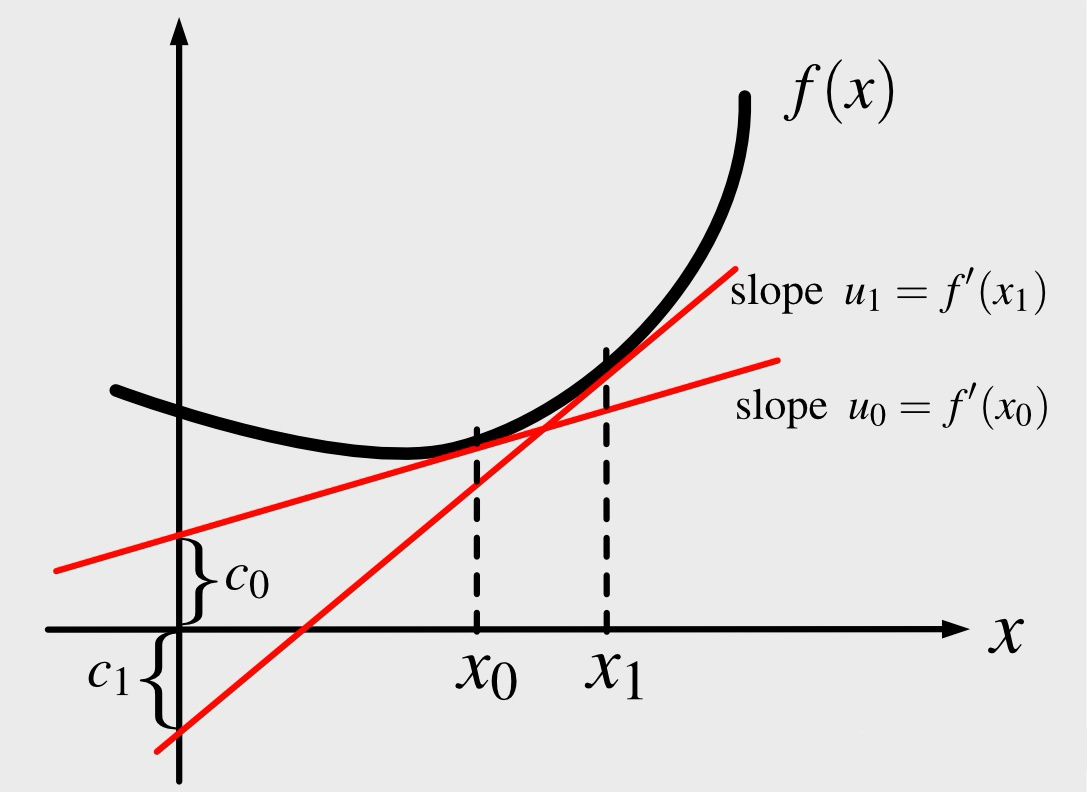
\includegraphics[scale=0.2]{./fig/Legendre Transform/1.png}
\end{figure}

一维情形下,如果我们想利用$f(x)$在某点$x_0$的切线斜率$u_0=f'(x_0)$确定$f(x_0)$,我们还需要知道这条切线的纵截距记为$c(x_0)$:
\[f(x_0)=f'(x_0)x_0+c(x_0)\]
我们也可以进一步将上式扩展到全定义域:
\[f(x)=f'(x)x+c(x)\]
由于切线斜率是已知的,所以这里我们更希望得到一个曲线斜率“表象”下的信息而非目前现有的坐标“表象”。因此,我们希望引入反函数
\[x=[f']^{-1}(u)\]
易知,这里我们要求$f':x \rightarrow u$是一个双射,故一般我们要求做$Legendre$变换的对象函数$f$是凸的,
当然也可以是凹的,不过一般物理上需要做$Legendre$变换的能量项都是凸的,故我们一般都默认$Legendre$变换是定义在凸函数上的。

明确上述要求后,我们继续往下
\[f([f']^{-1}(u))=u[f']^{-1}(u)+c([f']^{-1}(u))\]
这时,我们引入记号$\tilde{f}(u)$\textbf{称做$f(x)$的$Legendre$变换}:
\[\tilde{f}(u):=-c([f']^{-1}(u))=ux-f(x)\]

\begin{definition}[一维$Legendre$变换]
    定义$f(x)$为一个实变量的实值凸函数,我们称$\tilde{f}(u)$为$f(x)$的$Legendre$变换如果其满足
    \[\tilde{f}(u)=ux-f(x)\]
\end{definition}

函数的曲线$x \ vs. \ f(x)$表示的信息与由它在所有点的切线斜率$u=f'(x)$和截距$-\tilde{f}(u)$完全等价。
如果把图中所有点的的切线都画出来,它们描绘(切)出的曲线边缘就是$f(x)$的形状。
\begin{figure}[htbp]
    \centering
    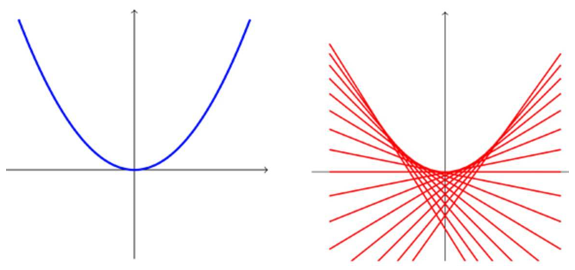
\includegraphics[scale=0.8]{./fig/Legendre Transform/2.png}
\end{figure}
所以说$Legendre$变换将点与线的信息关联起来,也称作对偶性($duality$)。
$f(x)$和$\tilde{f}(u)$互为$Legendre$变换,且$Legendre$变换具有对合性,即$\tilde{\tilde{f}}=f$。

$Legendre$变换是一个实变量的实值凸函数的对合变换,代数意义上,$Legendre$变换是一将向量空间($Vector \ space$)映射到对偶空间($Dual \ Space$)的双射;
在微分几何语言描述中它是切丛到余切丛的同构映射。

进而我们可以二维情形,给定二元凸函数$f(x,y)$,其全微分如下:
\[df=\frac{\partial f}{\partial x}dx+\frac{\partial f}{\partial y}dy:=udx+vdy\]

考虑表象变换$(x,y) \ \rightarrow \ (u,v)$:
\[\frac{\partial f}{\partial u}=\frac{\partial f}{\partial x}\frac{\partial x}{\partial u}+\frac{\partial f}{\partial y}\frac{\partial y}{\partial u}=u\frac{\partial x}{\partial u}+v\frac{\partial y}{\partial u}=\frac{\partial (ux)}{\partial u}-x+v\frac{\partial y}{\partial u}\]
\[\frac{\partial f}{\partial v}=\frac{\partial f}{\partial x}\frac{\partial x}{\partial v}+\frac{\partial f}{\partial y}\frac{\partial y}{\partial v}=u\frac{\partial x}{\partial v}+v\frac{\partial y}{\partial v}=u\frac{\partial x}{\partial v}+\frac{\partial (vy)}{\partial v}-y\]
易得
\[x=\frac{\partial (ux+vy-f)}{\partial u}:=\frac{\partial \tilde{f}}{\partial u}\]
\[y=\frac{\partial (ux+vy-f)}{\partial v}:=\frac{\partial \tilde{f}}{\partial v}\]

同样地,我们也可以定义n维$Legendre$变换。

\begin{definition}[n维$Legendre$变换]
    定义$f(x_1,x_2,\cdots,x_n)$为一个实变量的实值凸函数,我们称$\tilde{f}(u_1,u_2,\cdots,u_n)$为$f(x_1,x_2,\cdots,x_n)$的$Legendre$变换如果其满足
    \[\tilde{f}(u_1,u_2,\cdots,u_n)=\sum_{i=1}^nx_iu_i-f(x_1,x_2,\cdots,x_n)\]
    其中
    \[u_i=\frac{\partial f}{\partial x} \qquad x_i=\frac{\partial \tilde{f}}{\partial u} \qquad (i-1,2,\cdots,n)\]
\end{definition}

容易验证
\[d\tilde{f}=\sum_{i=1}^n(x_idu_i+u_idx_i)-df=\sum_{i=1}^nx_idu_i \qquad x_i=\frac{\partial \tilde{f}}{\partial u} \qquad (i-1,2,\cdots,n)\]

$Legendre$变换在热力学上有应用,其中一个例子就是四个热力学函数之间的转换,四个热力学函数的相互转化关系如下
\[U=U(S,V)\]
\[H=H(S,p)=U+pV \qquad F=F(T,V)=U-TS \qquad G=G(T,p)=H-TS=U+pV-TS\]
由
\[dU=TdS-pdV\]
可以得到其他函数的全微分
\[dH=d(U+pV)=TdS-pdV+pdV+Vdp=TdS+Vdp=dH(S,p)\]
\[dF=d(U-TS)=TdS-pdV-TdS-SdT=-SdT-pdV=dF(T,V)\]
\[dG=d(U+pV-TS)=TdS-pdV+pdV+Vdp-TdS-SdT=Vdp-SdT=dG(T,p)\]

进而可以得到$Maxwell$关系
\[dU=TdS-pdV \quad \Rightarrow \quad \left(\frac{\partial T}{\partial V}\right)_S=-\left(\frac{\partial p}{\partial S}\right)_V\]
\[dH=TdS+Vdp \quad \Rightarrow \quad \left(\frac{\partial T}{\partial p}\right)_S=\left(\frac{\partial V}{\partial S}\right)_p\]
\[dF=-SdT-pdV \quad \Rightarrow \quad \left(\frac{\partial S}{\partial V}\right)_T=\left(\frac{\partial p}{\partial T}\right)_V\]
\[dG=Vdp-SdT \quad \Rightarrow \quad \left(\frac{\partial S}{\partial p}\right)_T=-\left(\frac{\partial V}{\partial T}\right)_p\]

在经典力学中,拉格朗日量到哈密顿量的变换也是有$Legendre$变换完成的。
$Lagrangian$可以描述为$L=L(\mathbf{q},\dot{\mathbf{q}},t)$这里$q_i$、$\dot{q}_i$、$t$分别为广义坐标、广义速度和一维时间。利用$Euler-Lagrange$方程
\[\frac{d}{dt}\frac{\partial L}{\partial \dot{q}_i}=\frac{\partial L}{\partial q_i}\]
对$L$求全微分
\[dL=\sum_i\frac{\partial L}{\partial q_i}dq_i+\sum_i\frac{\partial L}{\partial \dot{q}_i}d\dot{q}_i+\frac{\partial L}{\partial t}dt
=\sum_i\frac{\partial L}{\partial q_i}dq_i+\sum_i\left[d\left(\frac{\partial L}{\partial \dot{q}_i}\dot{q}_i\right)-\dot{q}_id\left(\frac{\partial L}{\partial \dot{q}_i}\right)\right]+\frac{\partial L}{\partial t}dt\]

现引入广义动量$p_i$
\[\dot{p_i}=\frac{d}{dt}\frac{\partial L}{\partial \dot{q}_i}=\frac{\partial L}{\partial q_i}\]
则
\[dL=\sum_i\dot{p_i}dq_i+\sum_id\left(p_i\dot{q}_i\right)-\sum_i\dot{q}_idp_i+\frac{\partial L}{\partial t}dt\]
$Hamiltonian$是广义坐标、广义动量和时间的函数$H=H(\mathbf{q},\mathbf{p},t)$,利用$Legendre$变换
\[H(\mathbf{q},\mathbf{p},t)=\sum_ip_i\dot{q}_i-L(\mathbf{q},\dot{\mathbf{q}},t)\]
\[dH=\sum_id\left(p_i\dot{q}_i\right)-dL=\sum_i\dot{q}_idp_i-\sum_i\dot{p_i}dq_i-\frac{\partial L}{\partial t}dt\]

直接对$H$求全微分
\[dH=\sum_i\frac{\partial H}{\partial q_i}dq_i+\sum_i\frac{\partial H}{\partial p_i}dp_i+\frac{\partial H}{\partial t}dt\]
可得\textbf{$Hamilton$正则运动方程}
\[\dot{q}_i=\frac{\partial H}{\partial p_i} \qquad \dot{p}_i=-\frac{\partial H}{\partial q_i} \qquad (i=1,2,\cdots,n)\]
以及
\[\frac{\partial L}{\partial t}=-\frac{\partial H}{\partial t}\]
\textbf{注意:拉格朗日力学里广义坐标和广义速度是相互独立的,哈密顿力学里广义坐标和广义动量是相互独立的!}

\section{绝热表象和透热表象}